\documentclass[11pt,ngerman]{article}
\usepackage{geometry}
\usepackage[T1]{fontenc}
\usepackage[utf8]{inputenc}
\usepackage{babel}
\usepackage{lmodern}%get scalable font
\usepackage{titling}
\usepackage{relsize}
\usepackage{biblatex}
\usepackage{hyperref}
\usepackage{paralist}
\usepackage[table, dvipsnames]{xcolor}
\usepackage{booktabs}
\usepackage{setspace}
\usepackage{float}
\usepackage{graphicx}
\usepackage{listings}

% Link colors
\hypersetup{
    colorlinks,
    linkcolor={blue},
    citecolor={red},
    urlcolor={blue}
}

% inline code macro
\definecolor{lightgray}{gray}{0.9}
\lstset{
    showstringspaces=false,
    basicstyle=\ttfamily,
    keywordstyle=\color{blue},
    commentstyle=\color[grey]{0.6},
    stringstyle=\color[RGB]{255,150,75}
}
\newcommand{\inlinecode}[2]{\colorbox{lightgray}{\lstinline[language=#1]$#2$}}

% Code block settings
\definecolor{codegreen}{rgb}{0,0.6,0}
\definecolor{codegray}{rgb}{0.5,0.5,0.5}
\definecolor{codepurple}{rgb}{0.58,0,0.82}
\definecolor{backcolour}{rgb}{0.95,0.95,0.92}

\lstdefinestyle{mystyle}{
    backgroundcolor=\color{backcolour},
    commentstyle=\color{codegreen},
    keywordstyle=\color{magenta},
    numberstyle=\tiny\color{codegray},
    stringstyle=\color{codepurple},
    basicstyle=\ttfamily\footnotesize,
    breakatwhitespace=false,
    breaklines=true,
    captionpos=b,
    keepspaces=true,
    numbers=left,
    numbersep=5pt,
    showspaces=false,
    showstringspaces=false,
    showtabs=false,
    tabsize=2
}
\lstset{style=mystyle}

% double quotes macro
% usage: \quotes{arg1}  => in text: "arg1"
\newcommand{\quotes}[1]{``#1''}

\geometry{a4paper, top=25mm, left=25mm, right=25mm, bottom=20mm,
    headsep=10mm, footskip=12mm}

\renewcommand{\arraystretch}{1.5}

\pretitle{\begin{center}\linespread{1.5}\huge}
    \posttitle{\par\end{center}\vspace{0.5em}}

\begin{document}

    \title{SWEN1\\Praktikum 04 Design\\
        \vspace{1cm}
        \small{ZHAW  School of Engineering\\Klasse: IT18tb\_zh}
        \vspace{1.5cm}
    }
    \author{
        Huber, Patrick\\
        \small{huberpa4@students.zhaw.ch}
        \vspace{1.5cm}
    }
   \date{\today}

    \maketitle
    \newpage

    \tableofcontents
    \listoffigures
    \newpage

    \section{Praktikum Design}

    \subsection{Systemoperation 1 - registerUser}
     \inlinecode{Java}{registerUser(userData)} registriert einen neuen Benutzer, indem alle Daten in die Datenbank geschrieben werden.

        \subsubsection{Sequenzdiagramm registerUser(userData)}
        \label{sssec:Sequenzdiagramm_registerUser}
        \begin{figure}[H]
            \centering
            \makebox[\textwidth][c]{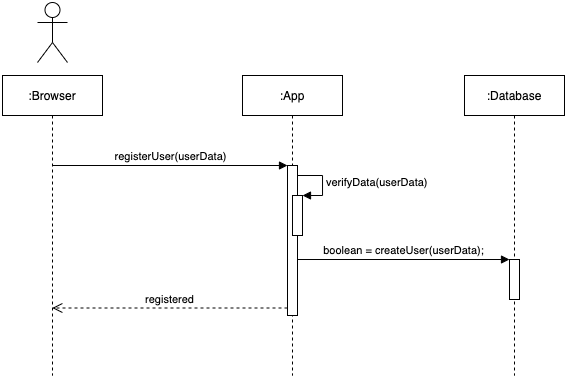
\includegraphics[width=0.95\textwidth]{figures/Sequenzdiagramm_registerUser.png}}
            \caption{UML Sequenzdiagramm - registerUser(...)}
            \label{fig:Sequenzdiagramm_registerUser}
        \end{figure}

     \subsection{Systemoperation 2 - loginUser(username, pass)}
     \inlinecode{Java}{loginUser(username, pass)} authentifiziert einen Benutzer gegenüber der Applikation, indem die eingegeben Daten mit den Daten aus der Datenbank verglichen werden.

         \subsubsection{Kommunikationsdiagramm}
          \begin{figure}[H]
             \centering
             \makebox[\textwidth][c]{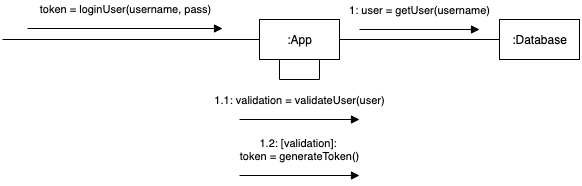
\includegraphics[width=0.95\textwidth]{figures/Kommunikationsdiagramm_loginUser.png}}
             \caption{UML Kommunikationsdiagramm - loginUser(username, pass)}
             \label{fig:UMLKommunikationsdiagramm_loginUser}
         \end{figure}

     \subsection{Design-Klassen-Diagramm}
     Ein Klassendiagramm existiert bereits für unseren Gameserver in Java. Jedoch wird die Authentifizierung nicht über Java gelöst und somit hat dieses Klassendiagramm nichts mit den zwei Systemoperationen zu tun. Es macht also wenig Sinn das Diagramm hier einzufügen.

\end{document}

